\section{Evaluation and Results}
\label{sec:evaluation}

We evaluate CodeGraph on SWE-bench Lite, a benchmark of 300 real GitHub issues paired with human-written fixes across 12 popular Python repositories. The task is file-level retrieval: given only a natural-language issue description and a repository, the system must rank source files by relevance and place the file modified in the human patch near the top.

\subsection{Evaluation Framework and Metrics}

SWE-bench Lite simulates a realistic retrieval scenario. The repositories are large, the issues use unstructured vocabulary, and the ground-truth patch is unambiguous. Our primary metric is \textbf{Recall@10}, representing the fraction of issues where the target file appears in the top-10 results. We also report Mean Reciprocal Rank (MRR) and the Zero-recall count (the number of issues where the target file does not appear in the top-10 at all). 

We compare CodeGraph against three baselines that together isolate the individual contributions of lexical matching, graph structure, and PPR ranking:
\begin{enumerate}
    \item \textbf{Random:} Files are ranked uniformly at random. This establishes the performance floor and calibrates the absolute scale of improvements.
    \item \textbf{BM25-only:} A sparse lexical retriever over the same entity corpus used for seeds. This baseline shares CodeGraph's lexical foundation while omitting the structural component, making it the most important point of comparison for measuring the value of graph-based propagation.
    \item \textbf{One-hop ego graph:} An unranked structural baseline that returns all neighbours within one hop of the seed nodes. This tests whether graph structure alone, without a ranking function, provides useful retrieval signal.
\end{enumerate}

\subsection{Performance Trajectory}

The initial configuration of CodeGraph achieved 42.0\% Recall@10, which underperformed the BM25-only baseline of 49.7\%. However, through systematic engineering of the seed stage, the final optimal configuration reached \textbf{74.0\% Recall@10}, an absolute improvement of 32 percentage points (see \Cref{tab:trajectory-results} and \Cref{fig:trajectory}).

\begin{table}[htbp]
    \centering
    \caption{Performance trajectory. Each row adds one intervention.}
    \label{tab:trajectory-results}
    \begin{adjustbox}{max width=\linewidth}
    \begin{tabularx}{\linewidth}{@{} >{\RaggedRight\arraybackslash}X >{\RaggedRight\arraybackslash}p{1.2cm} >{\RaggedRight\arraybackslash}p{1.2cm} >{\RaggedRight\arraybackslash}p{1.2cm} >{\RaggedRight\arraybackslash}p{1.6cm} @{}}
        \toprule
        \textbf{Configuration} & \textbf{R@5} & \textbf{R@10} & \textbf{MRR} & \textbf{Zero-recall} \\
        \midrule
        Weighted PPR (Initial Baseline)  & 37.0\% & 42.0\% & 0.228 & 174 \\
        Uniform PPR (Algorithm Refine.) & 55.3\% & 60.7\% & 0.344 & 118 \\
        + Improved Seeds (Seed Eng.) & 60.7\% & 72.3\% & 0.439 & 83 \\
        + Top-$k$ = 30 (Final Optimal)      & \textbf{60.7\%} & \textbf{74.0\%} & \textbf{0.442} & \textbf{78} \\
        \midrule
        \textit{BM25-only Baseline}      & 37.7\% & 49.7\% & 0.248 & 151 \\
        \bottomrule
    \end{tabularx}
    \end{adjustbox}
\end{table}

The improvement trajectory follows three stages:
\begin{enumerate}
    \item \textbf{Algorithm Refinement (+18.7pp):} Switching from confidence-weighted to uniform PPR restart closes the gap with BM25 and immediately surpasses it. When seeds are noisy or ambiguous, assigning them proportional weights amplifies false positives and misdirects the random walk. Uniform restart lets graph topology resolve the competition between seeds.
    \item \textbf{Seed Engineering (+11.6pp):} Implementing compound tokenization, an expanded BM25 corpus, and inverse-frequency weighting ensures that natural-language issue descriptions can be mapped to code entities reliably. This was the most impactful engineering intervention across all iterations.
    \item \textbf{Budget Adjustment (+1.7pp):} Increasing the candidate pool from $k=20$ to $k=30$ recovered a small band of instances where PPR correctly identified the target neighbourhood but ranked the gold file just outside the initial threshold.
\end{enumerate}

\begin{figure}[htbp]
    \centering
    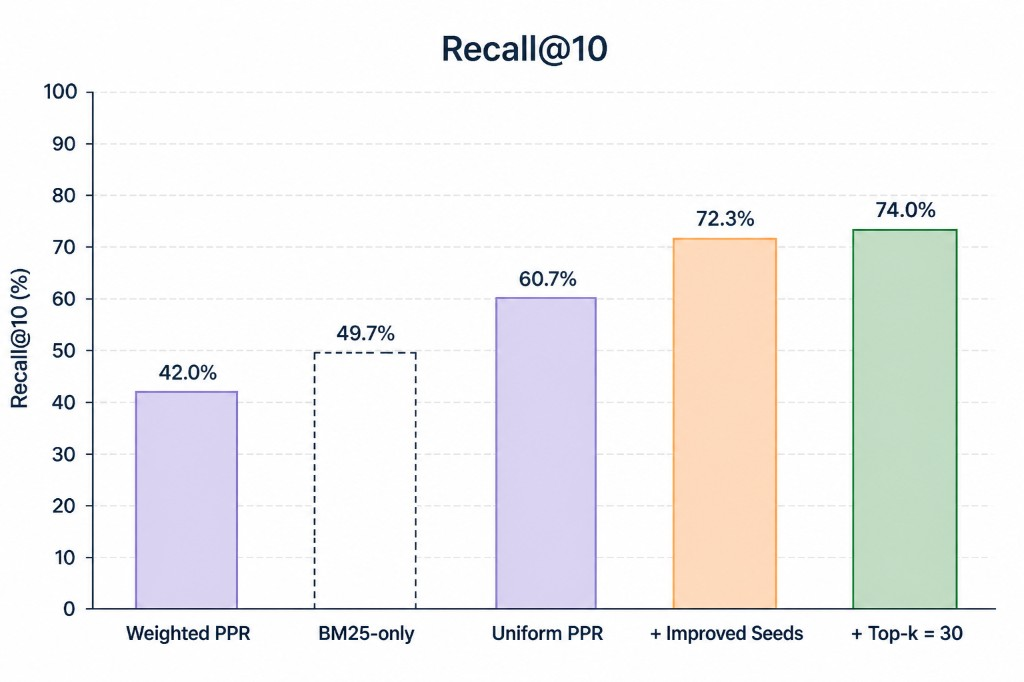
\includegraphics[width=\linewidth]{assets/recall_trajectory.png}
    \caption{Recall@10 trajectory. The gray bar (BM25-only) is shown for reference.}
    \label{fig:trajectory}
\end{figure}

\subsection{The Reachability Bottleneck}

A defining characteristic of CodeGraph's performance is its bimodal rank distribution: the target file almost always lands in the top-5 or does not appear in the top-10 at all. As \Cref{fig:bimodal} shows, only 5\% of instances fall into the intermediate band (ranks 6--10).

This pattern reveals a crucial insight: the retrieval ceiling is set by Reachability, not Ranking. If the system retrieves the target file at all, the PPR ranking places it highly. The zero-recall instances (78 cases) occur when no seed lies on a structurally connected path to the target file. When the seeds miss the relevant neighborhood, the graph has no signal to propagate. This diagnostic directly motivated our emphasis on seed quality improvements rather than advanced ranking heuristics.

\begin{figure}[htbp]
    \centering
    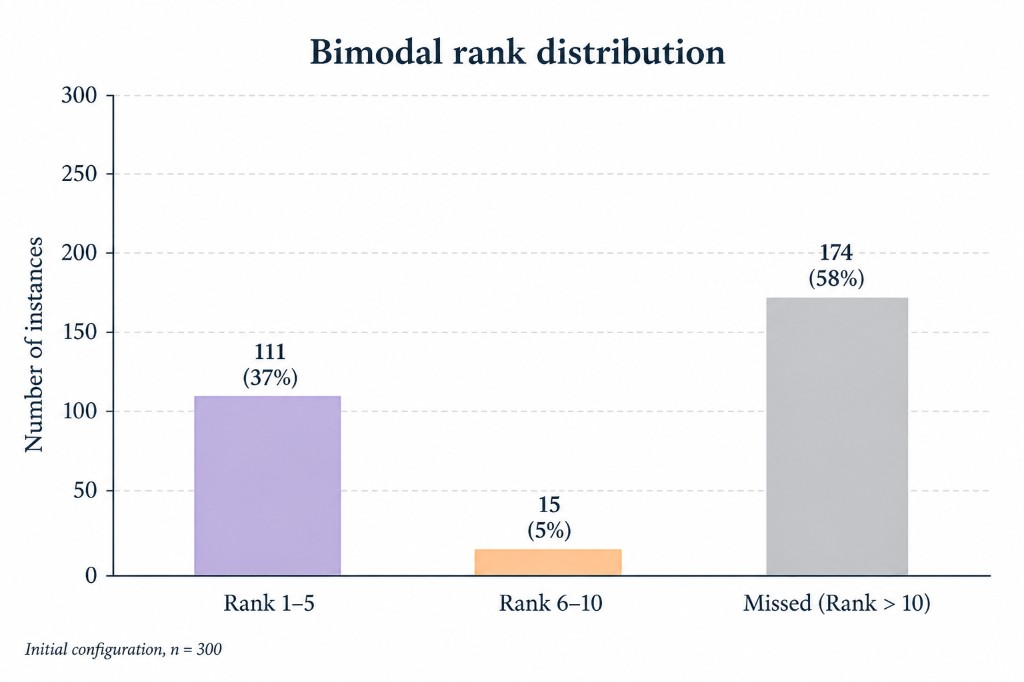
\includegraphics[width=\linewidth]{assets/bimodal_rank_distribution.png}
    \caption{Bimodal rank distribution for the initial configuration. The near-absence of intermediate ranks indicates that Reachability is the primary bottleneck.}
    \label{fig:bimodal}
\end{figure}
